\begin{figure}[h!]
	\hspace*{-2cm}\begin{tabular}{cc}
		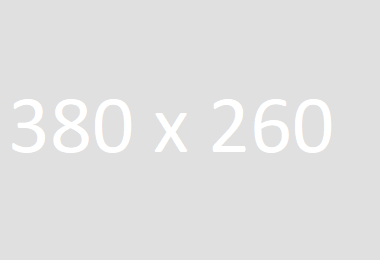
\includegraphics[width=70mm]{dummy.png} & 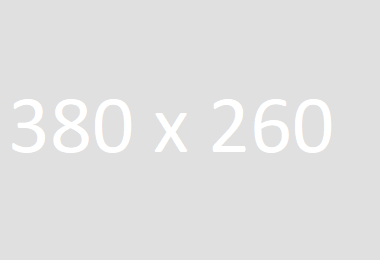
\includegraphics[width=70mm]{dummy.png} \\
		(a) Scatter Plot for each class & (b) Constant Density Curves and Decision Boundaries\\[4pt]
		
		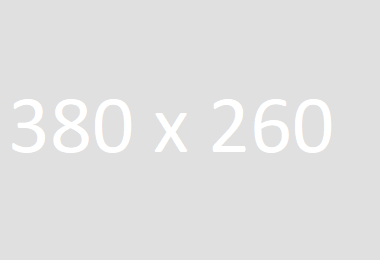
\includegraphics[width=70mm]{dummy.png} &   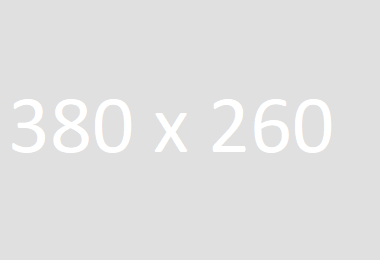
\includegraphics[width=70mm]{dummy.png} \\
		(c) Gaussian Distributions for each class and feature & (d) Confusion Matrix \\[4pt]
		
		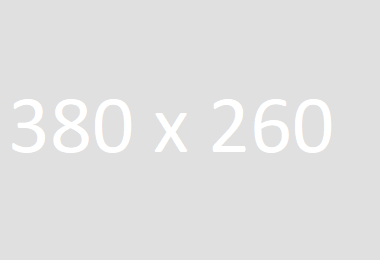
\includegraphics[width=70mm]{dummy.png} &   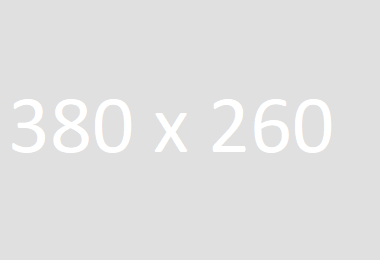
\includegraphics[width=70mm]{dummy.png} \\
		(e) ROC Curve & (f) DET Curve \\[4pt]		
		
		
		
		% To plot 5 images i 3x2 table
		\multicolumn{2}{c}{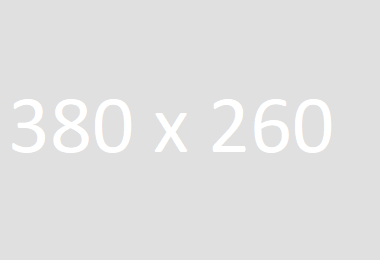
\includegraphics[width=70mm]{dummy.png} }\\
		\multicolumn{2}{c}{(e) ROC Curve}
		
	\end{tabular}\hspace*{-1cm}
	\caption{Summary of Linearly Separable Dataset}
\end{figure}